% =================================
%      Particle Accelerators
% =================================
\section{\review{Particle Accelerators}}

Particle accelerators are a relatively recent development, driven by the particle physics
field~\cite{bryant_brief_1994}. The first accelerators, at the beginning of the 20th century, were
able to accelerate particles up to energies of a few MeV using electric fields.

The Cockcroft Walton generator was powerful enough to split an atom for the first time in
1932~\cite{poole_cockcrofts_2007}, less than 100 years ago. Its design used capacitors and diodes
to double the voltage at each stage, with its main limitation being the breakdown voltage of the
capacitors. The Van de Graaff generator, created around the same time, was able to accelerate
particles up to tens of MeV. They are still in use today~\cite{lebois_rapport_2020} due to their
capability of producing a wide variety of ion beams with energies ranging from hundreds of KeV to
hundreds of MeV in the \textit{Tandem} form~\cite{hinterberger_electrostatic_2006}.

Radiofrequency generators with alternating electric fields and drift tubes, first created by 
Rolf Wideröe in the late 1920s, mark the beginning of modern accelerator
technology~\cite{vretenar_radio_2011}. Rapidly evolving, particle accelerators progressed from
accelerating particles to a few keV in linear accelerators to now TeV in circular accelerators,
called synchrotrons.

While single-beam synchrotrons can be used for fixed-target experiments, only a fraction of the
energy is available on impact. Dual-beam machines were more suitable for high energy physics
experiments. The first hadron collider, the ISR, was built at CERN in 1971 with an energy
of 62 GeV, taking its beam from the Proton Synchrotron (PS)~\cite{philip_cerns_2011}. 

Particle accelerators are still rapidly evolving. Several have been built in the past, and several
are now either under construction or in the design study phase. New acceleration and focusing
techniques are being developed, making the machines smaller. It is an exciting time for all fields
that might benefit from energetic particles, whether in fundamental research, medical, industrial or
security applications.


% =================================
%              CERN
% =================================

% --------------------------------
%          CERN Complex
% --------------------------------
\subsection{\review{The CERN Complex}}

CERN is a large laboratory located on the border of France and Switzerland, near Geneva. Although
well-known for discoveries in particle physics, studies are also conducted on medical applications,
biology, radiation hardness or material science.
Several accelerators are part of the accelerator complex, as illustrated in
\cref{fig:introduction:cern_complex}. A large number of fixed target experiments exist, whose
beams are delivered by various accelerators depending on their needs. These experiments are often
renewed~\footnote{Up to date information can be found on
\href{https://home.cern/science/experiments}{https://home.cern/science/experiments}.}.

The largest part of the CERN accelerator complex is the LHC. The LINAC4, PSB, PS and SPS
accelerators serve as pre-injectors to the LHC, taking priority over their other experiments.

\begin{figure}[!htb]
    \centering
    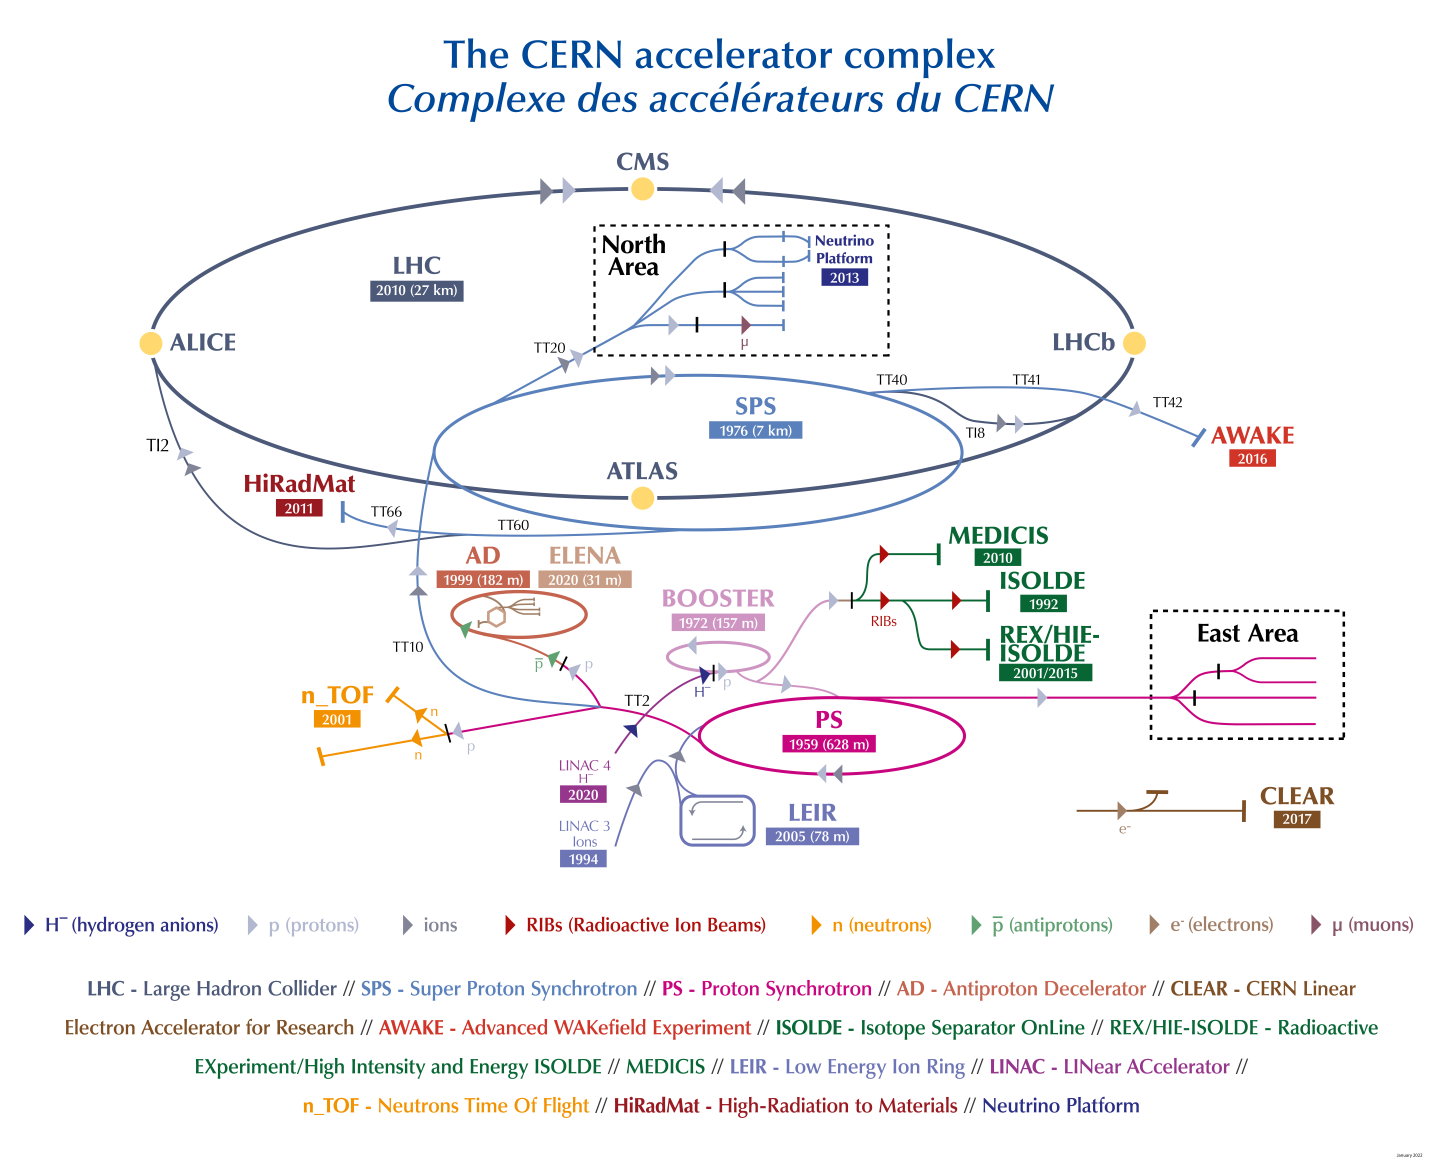
\includegraphics[width=1\textwidth]{images/cern_complex.png}
    \caption{Schematic illustration of the accelerator complex at CERN. Most accelerators are both
    used as injectors for the LHC or to provide beams to fixed target
    experiments~\cite{noauthor_cern_2022}.}
    \label{fig:introduction:cern_complex}
\end{figure}


% --------------------------------
%              LHC
% --------------------------------
\subsection{\review{The Large Hadron Collider}}

The Large Hadron Collider (LHC) is a circular particle accelerator primarily designed to collide
protons for fundamental particle physics research. It can also occasionally collide ions such as
oxygen or lead for specific studies. At the time of writing, in 2024, it holds several records,
such as being the largest and most powerful accelerator in the world, at nearly 27 km long. The LHC
is composed of two beam pipes, capable of accelerate two particle beams from an injection energy
of $450$ GeV to an energy of $6,800$GeV, before colliding them in four detectors: ATLAS, CMS, Alice
and LCHb.

Well-publicized, the LHC is often depicted via its superconducting dipole magnets, housed in blue
cryostats, aimed at cooling the coils. \Cref{fig:3d_cut_dipole} shows a 3D cut of such magnets. The
LHC is mostly composed of these \textit{main} dipoles, holding $1,232$ of them, each about 14 meters
long. Superconducting materials like niobium-titanium (NbTi) are utilized, as conventional materials
such as copper would melt under the current strain. Around $12,000$ amperes are supplied to generate
the magnetic fields necessary for bending the trajectory of the particles. These particles travel
at nearly the speed of light ($99.99999905\%$ of it), effectively going around the tunnel about
$11,200$ times per second.

\begin{figure}[!htb]
    \centering
    \includegraphics[width=0.8\textwidth]{chapters/01_Introduction/images/lhc_3D_cut.png}
    \caption{3D cut of a main LHC dipole~\cite{noauthor_cern_nodate}. Both beam pipes can be seen
    surrounded by the coils, strongly clamped by the yokes.}
    \label{fig:3d_cut_dipole}
\end{figure}


% -------------------------------
%   Straight Sections and Arcs
\subsubsection{\mread{Straight Sections and Arcs}}

The LHC is not a perfect circle. It is indeed composed of four \textit{straight} sections, called
the \textit{Interaction Regions} (IPs) where detectors or specific instrumentation are placed.
Connecting those sections, the \textit{arcs} are where the majority of the magnets and their
correctors are located, along with some instrumentation like beam position monitors.
\Cref{fig:introduction:lhc_irs} shows the arcs as well as the purpose of each straight section,
housing either specific instrumentation or detectors.

\begin{figure}[!htb]
    \centering
    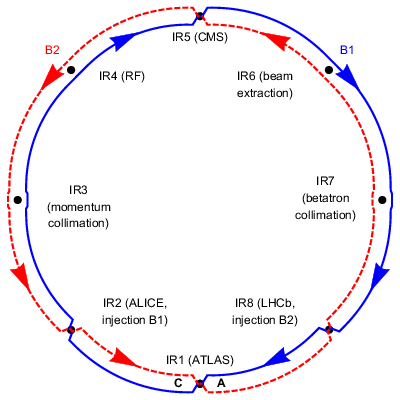
\includegraphics[width=0.5\textwidth]{./images/irs.png}
    \caption{Schematic of the LHC layout.}
    \label{fig:introduction:lhc_irs}
\end{figure}


% -------------------------------
%          Arc Cells
\subsubsection{\mread{Arc Cells}}

Each arc is made up of 23 cells. Magnets are organized in a standard FODO structure
(see \ref{section:courant_snyder}), as shown in \cref{fig:introduction:lhc_arc_cell}.
\textit{Dipoles} are responsible for bending the trajectory of the particles. Their associated
correctors, the orbit correctors, mitigate any possible drift in the path.
\textit{Quadrupoles} are used to control the beam size along the ring. Their effect is focusing in
one plane and defocusing in the other. Their associated correctors control the oscillations of the
beam (see tune, \ref{section:courant_snyder}) and possible field imperfections.
\textit{Sextupoles} correct chromaticity, a misfocus from quadrupoles due to particles having
a different momentum than the reference particle.
\textit{Octupoles} are used to stabilize the beam by introducing Landau
Damping~\cite{gareyte_landau_1997}. The associated correctors correct higher-order chromaticity
effects as well as amplitude-dependant tune shifts.
\textit{Decapoles} correctors aim at correcting an even higher chromaticity order.

\begin{figure}[H]
    \centering
    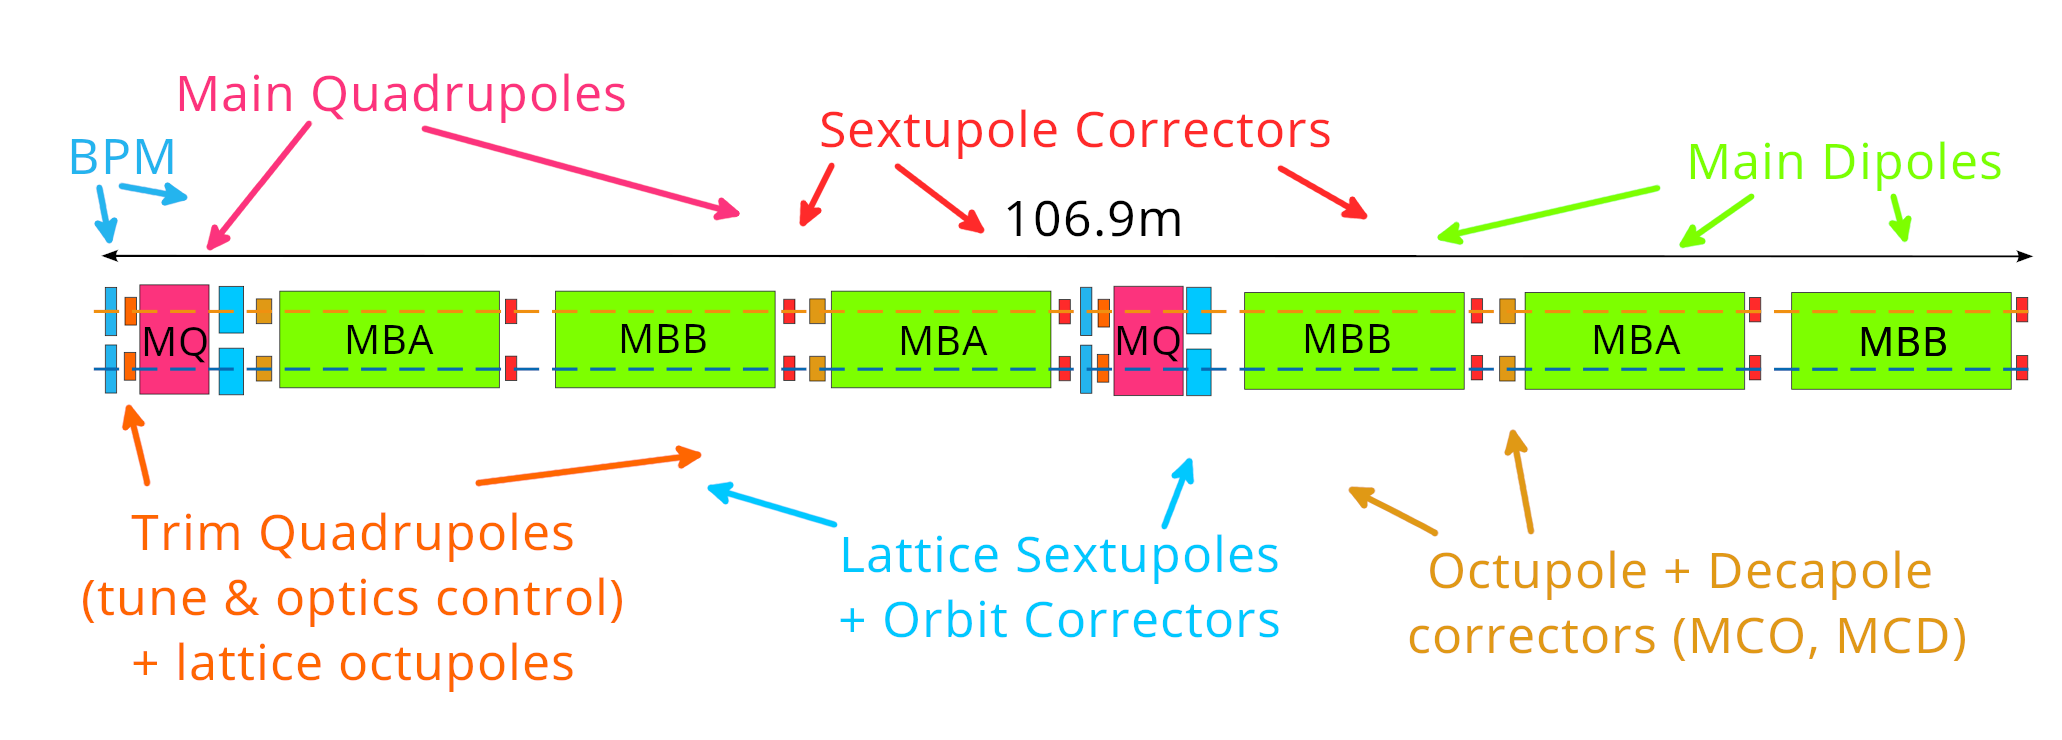
\includegraphics[width=1\textwidth]{./images/lhc_cell.png}
    \caption{Schematic of an LHC Arc cell~\cite{bruning_lhc_2004}.}
    \label{fig:introduction:lhc_arc_cell}
\end{figure}



% -------------------------------
%            Cycles
\subsubsection{\mread{Cycles}}

During the operation of the LHC, the machine goes through several states, each defined for specific 
scenarios~\cite{wenniger_lhc_2019}.

A common example is the operational cycle of the LHC, illustrated in \cref{fig:cern_complex:cycle}.
Initially, the magnets are pre-cycled~\cite{bottura_pre-cycles_2010} without any beam circulating,
to get them back to a reproducible state. Their current is then increased to accept particles at the
injection energy of 450GeV.  To verify the machine's proper functioning, a probe bunch of reduced
intensity is first injected The number of bunches and their intensity are then gradually increased
to attain the desired scheme needed for collisions, which varies throughout the year based on
experimental demands. The number of bunches and their intensity can be adjusted as needed to ensure
the machine's safety. A common scheme in 2024 is to inject about 2350 bunches with around $10^{11}$
particles each for collisions.  Optics measurements, due to their destructive nature, typically use
between one and three \textit{pilot} bunches at a lower intensity of $10^{10}$ particles.

The magnets' current is then ramped along with the voltage in the RF system, to accelerate particles
to an energy of 6.8 TeV. During this process, the beam is first squeezed at the Interaction Points.
After completing the ramp-up, a second pass is performed to achieve a $\beta* = 30$cm at the ATLAS
and CMS experiments, resulting in a smaller beam size. Crossing-angles are then introduced to make
the beams collide.

\begin{figure}[!htb]
    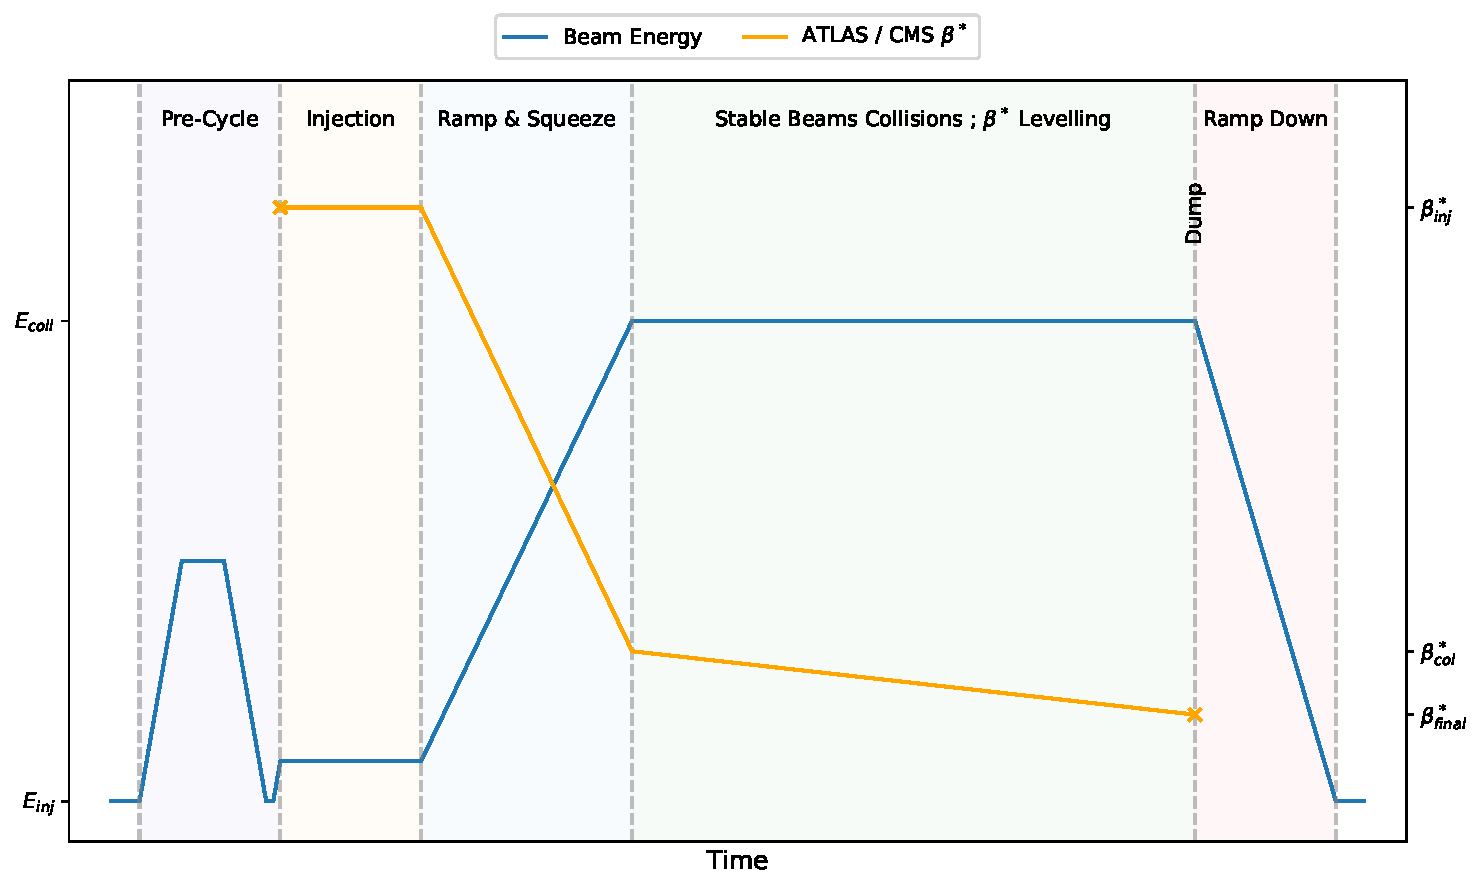
\includegraphics[width=\textwidth]{./images/lhc_cycle.pdf}
    \caption{Simplified illustration of a standard LHC cycle. Courtesy of Félix
    Soubelet~\cite{felix_soubelet_local_2023}.}
    \label{fig:cern_complex:cycle}
\end{figure}


% -------------------------------
%   Harmonics and Field Errors
\subsubsection{\review{Magnetic Fields}}

The magnetic fields of the LHC are created via the coils of the magnets. Real-life magnets never
have a single field as one would like. Instead, so called \textit{allowed harmonics} exist due to
the geometry of the coil. As such, the main dipoles of the LHC can exhibit fields similar to
sextupoles, decapoles, decatetrapoles and so on~\cite{deniau_magnetic_2009}. Manufacturing
imperfections also add fields errors outside of the scope of the allowed ones. Dipoles are indeed
found to generate octupolar field errors.

During the design of the LHC, the main dipoles have been identified to generate significant field
errors. Magnetic measurements of those various fields were thus taken and magnetic tables built
based on real-life magnets nowadays installed in the machine. Those magnetic tables, computed for
each LHC configuration by \textit{WISE}~\cite{p_hagen_wise_2006} are used by simulation softwares.
Predictions of field errors and compensating strength for the correctors is computed by the Field
Description for the LHC (\textit{FiDeL}, \cite{noauthor_fidel_2021}). FiDeL is used in the LHC
control system in operation to steer the beams.

%\begin{figure}[H]
    %\centering
    %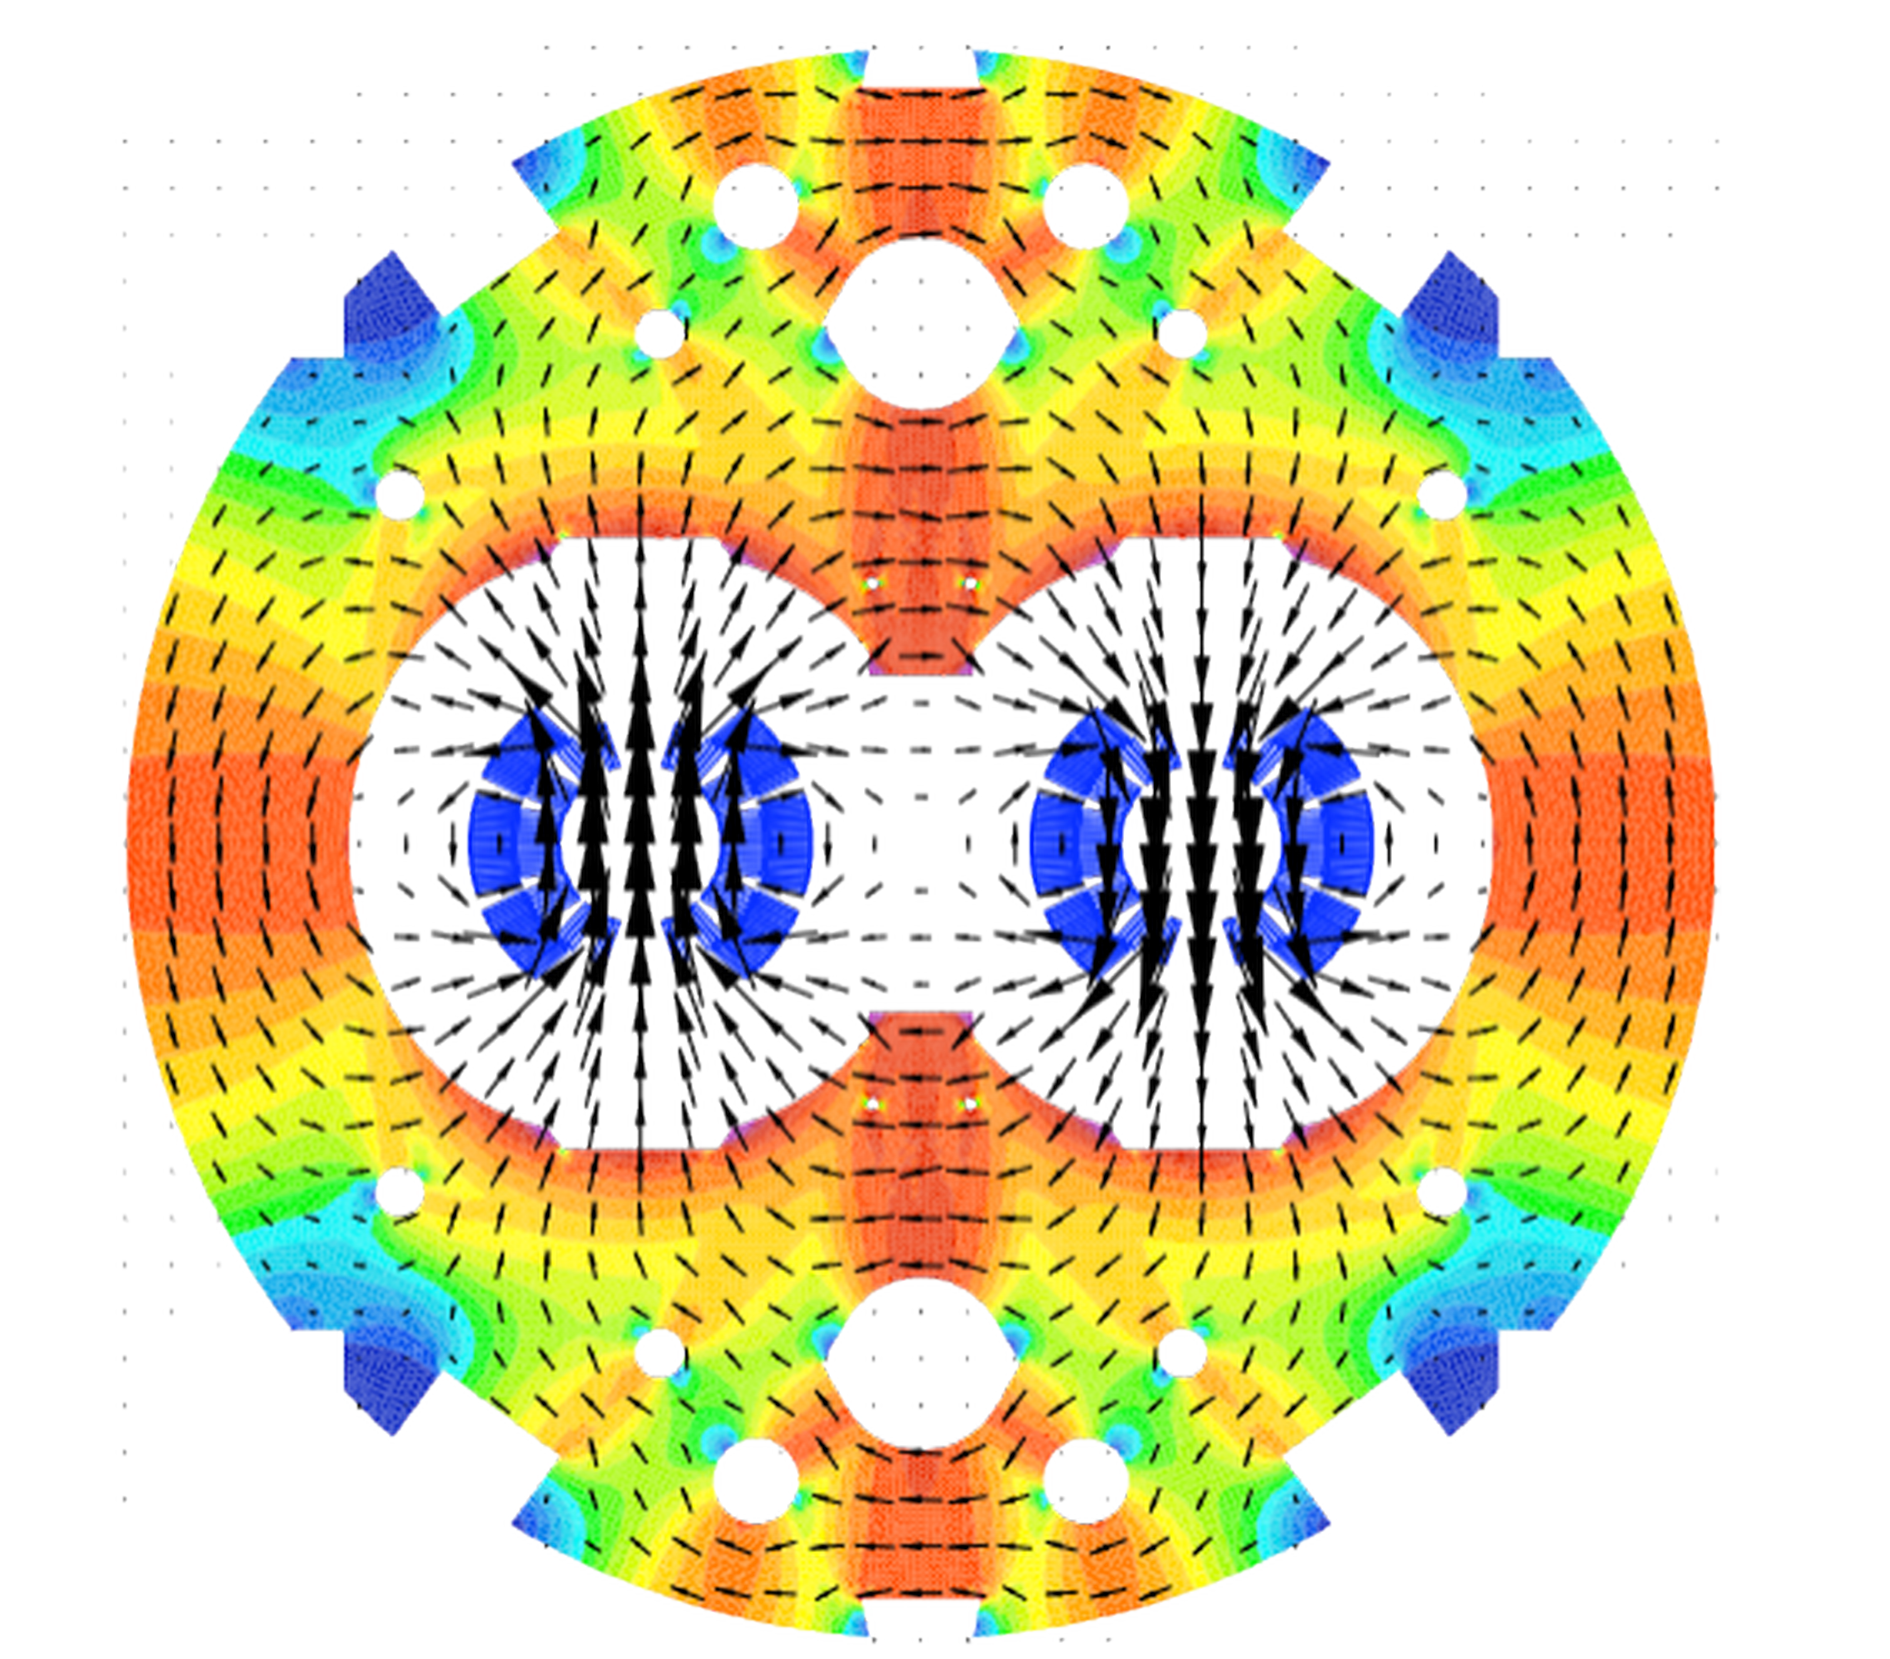
\includegraphics[width=0.5\textwidth]{./images/main_dipole_fields.png}
    %\caption{Magnetic field in a dipole magnet~\cite{deniau_magnetic_2009}.}
    %\label{fig:decapoles:magnetic_field_dipole}
%\end{figure}